\documentclass[nofilelist,dvipsnames]{cslthse-msc}
% to show a list of used packages at the end of the document, delete the nofilelist option
%\documentclass{cslthse-msc}
\usepackage[utf8]{inputenc}
\usepackage[english]{babel}
\usepackage{amsmath}
\usepackage{amsthm}
\usepackage{graphicx}
\usepackage[titletoc, header, page]{appendix}
\usepackage{transparent}
\usepackage[
	backend=biber,
	style=numeric,
	sorting=none,
]{biblatex}
\addbibresource{report.bib}
\usepackage{parskip}
\usepackage{textcomp}

% used to display the used files at the end. Select nofilelist as a package option to disable this
%\listfiles % initialize

%\geometry{showframe}
%better like this?
%\student{Flavius Gruian}{Flavius.Gruian@cs.lth.se}
\student{Stefan Eng}{atn08sen@lu.se}

\thesisnumber{LU-CS-EX: 2020-XX} % Birger Swahn will provide this number to you, once the thesis is ready for publication

\title{
  Usability testing on the web; Measuring how design impacts task performance
  times.
}

%\onelinetitle
%\twolinestitle
\threelinestitle
%\fourlinestitle

%\subtitle{A {\LaTeX} class}
\company{MASSIVE}
\supervisors{
  John Deer, \href{mailto:jdeer@company.com}{\texttt{jdeer@company.com}}
}{
  Don Jeer, \href{mailto:djeer@xy.lth.se}{\texttt{djeer@xy.lth.se}}
}
\examiner{Jane Doe, \href{mailto:jane.doe@cs.lth.se}{\texttt{jane.doe@cs.lth.se}}}

\date{\today}
%\date{January 16, 2015}

\acknowledgements{
}

\theabstract{
}

\keywords{
	Usability testing,
	Web-application,
	Flask,
	HTML
}

\begin{document}
\renewcommand{\bibname}{References}

\makefrontmatter
\newcommand{\todo}[1]{\textcolor{blue}{\textbf{TODO:} #1}}
\newcommand{\todoMaybe}[1]{\textcolor{OliveGreen}{\textbf{?TODO:} #1?}}
\newcommand{\eatdot}[1]{}
\newcommand{\ctitle}[1]{\citetitle{#1}\cite{#1}}
\newcommand{\varHere}[1]{\input{vars/#1.txt}\unskip}
\newcommand{\checkTruth}[0]{\textcolor{red}{(?)} }
\newcommand{\findref}[0]{\textcolor{orange}{[!]}}%
\newcommand{\todoInsert}[1]{\textcolor{purple}{\textit{<insert #1 here>}}}%

\chapter{Introduction}

  As the gaming industry continue to grow{\findref\findref} so do the reported
  number of stress-related issues reported by the people working in the
  sector{\findref\findref\findref}. The initial idea for this report came from a managers
  observation that co-workers would abandon the digital communication software
  for a more hands-on approaches, such as post-it notes on a whiteboard, when
  the pressure got to a certain point.

  Asking why, people stated that the software they were supposed to use for
  communicating and propagating the projects status throughout the team got in
  their way. Which is why they opted to use post-it notes, even though it has
  significantly worse communication bandwidth and is less accessible,
  at-least-it-works\texttrademark.

  \section[MASSIVE Entertainment | A Ubisoft studio]{MASSIVE}

  {\vspace{-0.7cm}{\hspace{1.85cm}\small MASSIVE ENTERTAINMENT | A UBISOFT STUDIO}}

    \todo{Expand section.}

  \section{Why usability testing?}

    Initially, the plan was to make interface changes to the organization-software
    itself, but a question remained, how do you prove that it actually makes a
    difference?

    \todo{Describe why usability testing, add scaling problem.}

  \section{Usability testing}

    \subsection{Introduction}

      Usability is traditionally done in person with the \textit{over the
        shoulder} method which gives a good insight of what a participant does
      during a test. Further more, if the \textit{thinking out aloud - method} is
      utilized correctly, the test-moderator should have a good insight into the
      participant thought-process during the test.

    \subsection{Evolution and state of the art}

      While effective\checkTruth this method scales poorly with a one to one ratio
      between moderator and test participant. This project investigates the
      possibility of alleviating this scale constraint by utilizing a internet
      based platform to conduct usability tests of user interfaces online.

      \todo{Expand this section.}

  \section{Running usability tests at larger scales}

    \todo{Expand this section.}

	\section{Report goals}

		\begin{enumerate}
			\item{Create a web based platform for usability testing.}
			\item{Run one or several interface tests with real users on the platform.}
			\item{
				Verify that the collected data shows a significant\checkTruth impact on the studied
				variable(s) when parameters are changed. \todoMaybe{Shorten}
			}
		\end{enumerate}

	\section{Literary scope}

		This report draws and builds on information from the fields of usability
		testing, web design and interaction design.

		Specifically, \ctitle{citeHandbookUsability} and
		\ctitle{citeUsabilityTestingEssentials}, provide a contrast between
		traditional and modern approaches to usability testing and how to perform
		them.

		\ctitle{citeDonMakeMeThink} provides a concise and interesting
		summary of no-nonsense approaches to web design from a usability perspective.
		Last but not least \ctitle{citeTheDesignOfEverydayThings} introduces
		both \textit{user-centered-} and \textit{interaction-design} together
		with the concept of \textit{affordances},

	  %Introduction to user interface design and usability testing? \\
	  %
		%Figure out how much of an impact different design aspects have on tasks
		%that require distinguishing one element from another. And doing it in a
		%decentralised manner based on web-application. \\
	  %
	  %Don't make me think -> webdesign. \\
	  %Design of everyday things -> webdesign. \\
	  %Report based on distances / colors -> webdesign. \\
	  %Usability-testing guide -> webapp suggesting + other. \\


	\chapter{Approach}

		\section{Method}

      This section expands on the methodology behind the initial concept and
      creation of the testing platform, as well as the process of generating
      and evaluating data from the usability tests performed by the participants.

      \subsection{Software development methodology}

        The goal was to adopt an agile development process{\findref} for the
        creation, evaluation and improvement of the usability testing platform.

        \begin{figure}[h!]
          \centering
          \includegraphics{figures/method.pdf}
          \caption{Concept, development, testing and improvement cycle.}
        \end{figure}

        This methodology is centered around creating a minimal
        working prototype{\findref} that is put in front of real users as soon
        as possible. The feedback data generated by the users should then be
        feed back into the design to improve the next prototype version, which
        is tested again. This cycle should then be repeated until either the
        software is satisfactory or the time is up.

%      The goal was to perform several full iteration cycles, but in the
%      end
%      While this was the goal, it only completed one whole full cycle, with
%      smaller iterations within the larger cycle. \todo{Reword}

      \subsection{Defining the initial concept}

        In order to perform usability tests that can be measured and validated,
        there needs to something for users to interact with. Since the subject
        of communication under pressure was the initial focus, the suggestion
        of helping managers reduce the stress for their team came up.

        After interviewing a couple of managers, the following ideas were
        gathered:

        \begin{itemize}
          \item{
            An easy way to see if a co-worker is assigned more work than they
            have available hours.
          }
          \item{
            Calendar overview where it is possible to determine if there are
            hot-spots where lots of results need to be produced at the same
            time.
          }
          \item{
            A concise way to identify if there are critical tasks that, if
            delayed, would delay other tasks that depend on it.
          }
          \item{
            The possibility to identify a group or teams strengths and assign
            task types accordingly.
          }
        \end{itemize}

      \subsection{Paper prototypes for a first-draft interface}

        Even though the initial interface setup was very bare-bones, it was
        still important to get it in front of users, in this case, test
        participants, as soon as possible.

        \begin{figure}[h!]
          \centering
          \begin{minipage}{.49\textwidth}
            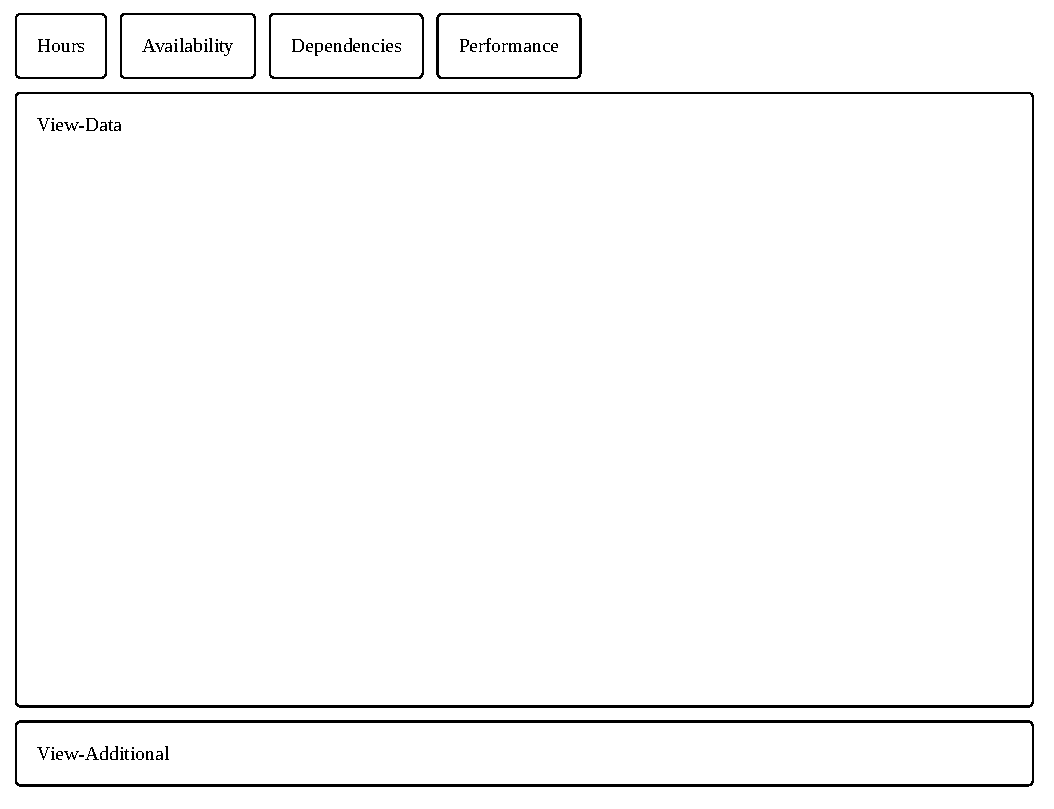
\includegraphics[width=\linewidth]{ui11.pdf}
          \end{minipage}
          \begin{minipage}{.49\textwidth}
            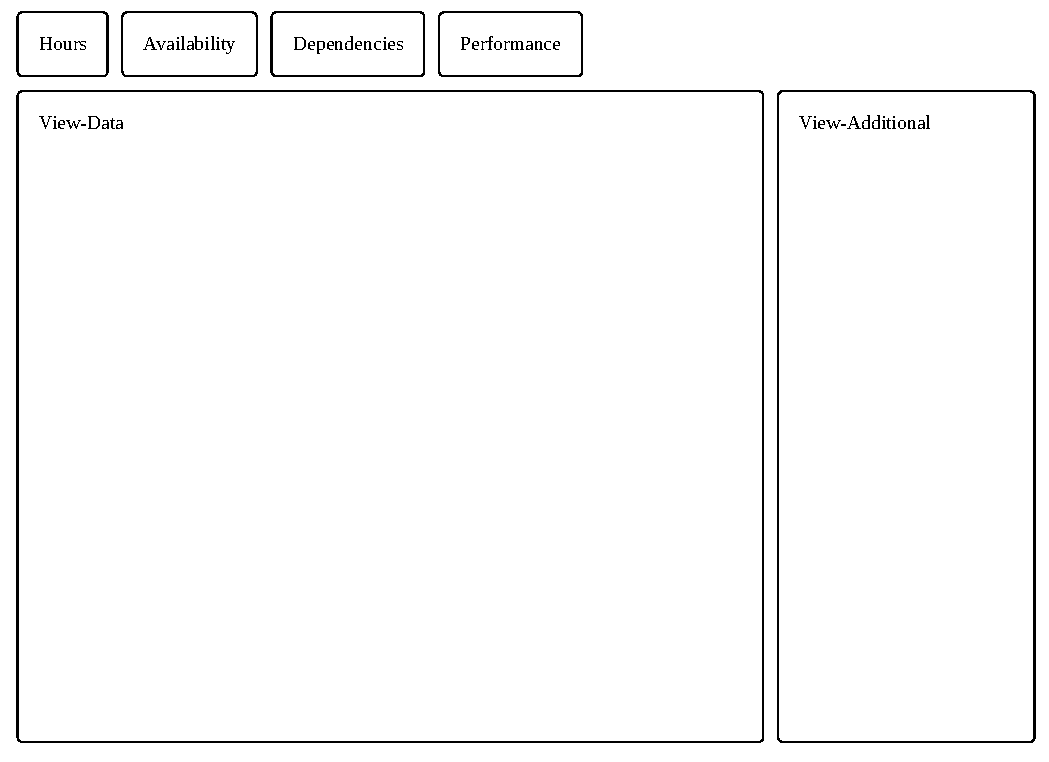
\includegraphics[width=\linewidth]{ui12.pdf}
          \end{minipage}
          \begin{minipage}{.49\textwidth}
            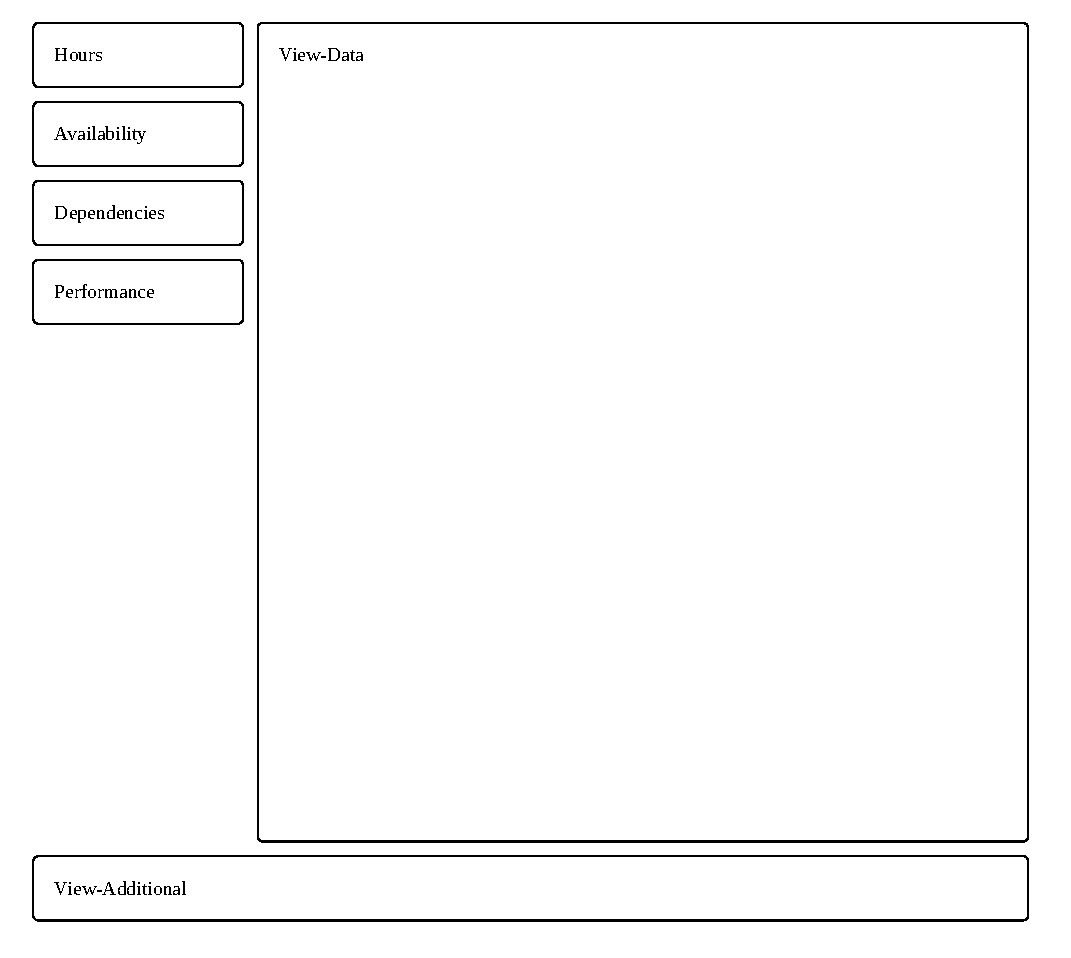
\includegraphics[width=\linewidth]{ui13.pdf}
          \end{minipage}
          \begin{minipage}{.49\textwidth}
            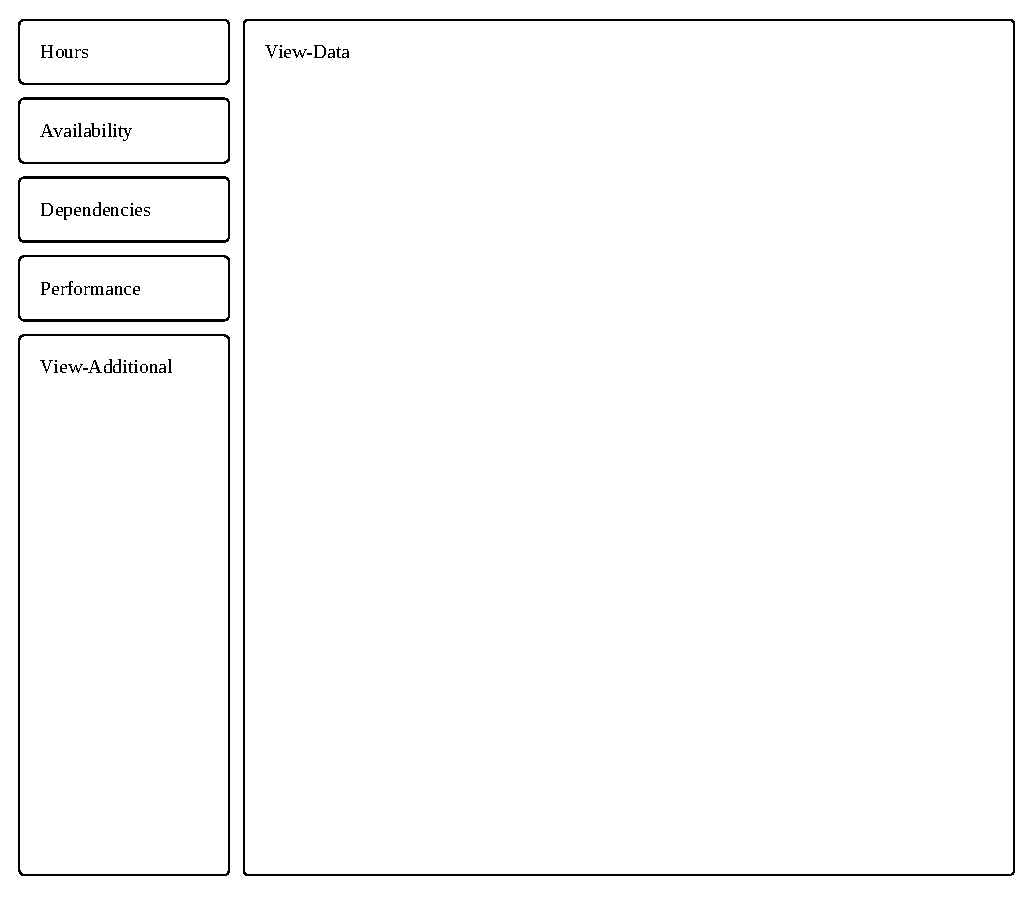
\includegraphics[width=\linewidth]{ui14.pdf}
          \end{minipage}
          \caption{Interface drafts 1.1, 1.2, 1.3 and 1.4.}
        \end{figure}

        \todoMaybe{These figures should probably be under result?}

        Four mock-up interfaces were created based on \todoInsert{part about
          ui design reference} and presented to five\checkTruth colleagues for
        evaluation. The evaluation was conducted as an in-person interview
        where the interviewee were asked to voiced their thoughts out aloud.
        After the initial reaction and thought about each of the designs, the
        interviewee was asked to pick, according to them, the most suitable
        design.

        After the initial pick, the interviewee was presented with
        \todoInsert{part about ISO-standard design}, which they had to arrange
        in order of most to least important according to their own views.
        After prioritizing the different design attributes, the participant was
        again asked to pick what they felt was the most suitable design.


        \todo{Expand with information about ISO design standard}

      \subsection{Gathering relevant test data}

        There is a two-fold goal that the collected test-data needs to solve:
        \begin{itemize}
          \item{
            Generate a quantifiable value that can be tracked in order to
            evaluate the participants performance during tests.
          }
          \item{
            Aggregate participant feedback about the platform in order to
            improve the next version.
          }
        \end{itemize}

        The first problem is solved by sticking with a established tradition
        within usability testing\findref\findref, measuring completion time.
        In order to keep track of their test-runs, participant are assigned an
        anonymous id-string after acknowledging that they have read the initial
        information. The anonymous id is registered as used in the database
        and the id is stored in the participants browsers web-session.

        As a participant starts a new task, the database will register the
        start-time and link it to the aforementioned anonymous id. If the
        participant completes the task, the stop-time will be recorded in the
        same database post, and the difference between these two values will be
        used as the time for task completion.

        Acquiring feedback data is done through a post-test survey with ten set
        questions (1-5) and a free-from dialog box for additional input.
        \todo{Expand and reword last section}


      \subsection{Evaluating impact and effectiveness}

        \todo{expand this section}

%			Results by measuring the time and showing graphs + statistical grouping /
%			analysis.

		\section{Theory}

			The theory contains color-theory and the experience from managerial
			positions.

			\subsection{Information presentation and color}

			\subsection{Representative simplified task models}

			\subsection{Measuring time to task completion}

			\subsection{Threshold for failure}


		\section{Implementation}

			Writing a web-application with Flask + python + sqlite3.
			HTML5 and CSS with a dab javascript.

			\subsection{Platform software stack}

			\subsection{Interface creation}

			\subsection{Variable challenges}

      \addtocontents{toc}{\pagebreak}
	\chapter{Evaluation}

		\section{Results}

			\subsection{Participation, test runs and success ratio}

				The test-site went live 2020-01-24 and the link was initially shared
				through Facebook. On 2020-01-27 the link was shared on
				the MASSIVE internal mailing list, boosting the participation
				significantly. In a total,
				\varHere{totalParticipants} participants got past the initial information
				page over a five day period.

				\begin{figure}[h!]
					\centering
					\includegraphics{figures/participantsOverTime.pdf}
					\caption{Total registered participants over time.}
				\end{figure}

				In total \varHere{totalTests} tests were run, where
				\varHere{totalTestsCorrect} were answered correctly,
				\varHere{totalTestsUncompleted} never produced an answer, leaving
				\varHere{totalTestsIncorrect} incorrect answers. Looking only on the test
				runs without any user- or task-correlation, the chance that any given test run
				produces the correct answer is $\sim$\varHere{varTotalRatioSuccess}\%.

				\begin{figure}[h!]
					\centering
					\includegraphics{figures/runsOverTime.pdf}
					\caption{Total number of tests run overt time.}
				\end{figure}

			\subsection{Test runs per user and participation activity}

				The number of recommended test was five, which when completed, allowed
				the participants to continue to the final survey. However, there was
				nothing stopping each participant from doing more or less than the
				suggested number.

				\begin{figure}[h!]
					\centering
					\includegraphics{figures/testsPerUser.pdf}
					\caption{Number of users that performed a specific number of tests.
						\textit{(Tabulated data available in appendix.)}}
				\end{figure}

        \ \\
        Of the \varHere{totalParticipants} number of participant sessions started,
        \varHere{valNumAnyTestsRun}
%				(\varHere{valNumAnyTestsRunP})
        of them ran at least one test, which means \varHere{valTestNoTests} ran
        no tests. Further more, \varHere{valTestsFiveToTen} completed between
        five and nine tests, and \varHere{valTestsElevenOrMore} completed ten or
        more.
%				(\varHere{valNumFiveOrMoreTestRunP})

      \subsection{Test types, test order and task distribution}

        Since the participants were free to choose any combination of tests,
        it's interesting to know which of the tasks were run the most.

				\begin{figure}[h!]
					\centering
					\includegraphics{figures/testsRunPerTask.pdf}
					\caption{Test run distributed on task-types.}
				\end{figure}

      \todo{
        Continue exploring the data, time distribution? Which task was failed
        the most? Are there thresholds in the variables where tasks start to
        fail more often? Is there a most preferable order to do the tasks?
        Which task is the most popular in the 5-run category? ...
      }


		\section{Discussion}

			\subsection{Possible improvements}

			\subsection{Threats to validity}

%				network latency?
%				multiple runs with same person?



	\chapter{Conclusions}

		Did it have an significant impact? Was the web the correct platform? What
		could be done better over the internet? Recording screen and voice?
		(Javascript, since it's already used, pull up some statistics?)

	% Should use consistent formatting when it comes to Names ("FirstName LastName", or "F. LastName")
	\makebibliography{report}

	%make sure we're on even page with the pop-sci
	\checkoddpage
	\ifoddpage
	\else
		 \newpage
		 \thispagestyle{empty}
		 \mbox{ }
	\fi
	%\begin{appendices}
	%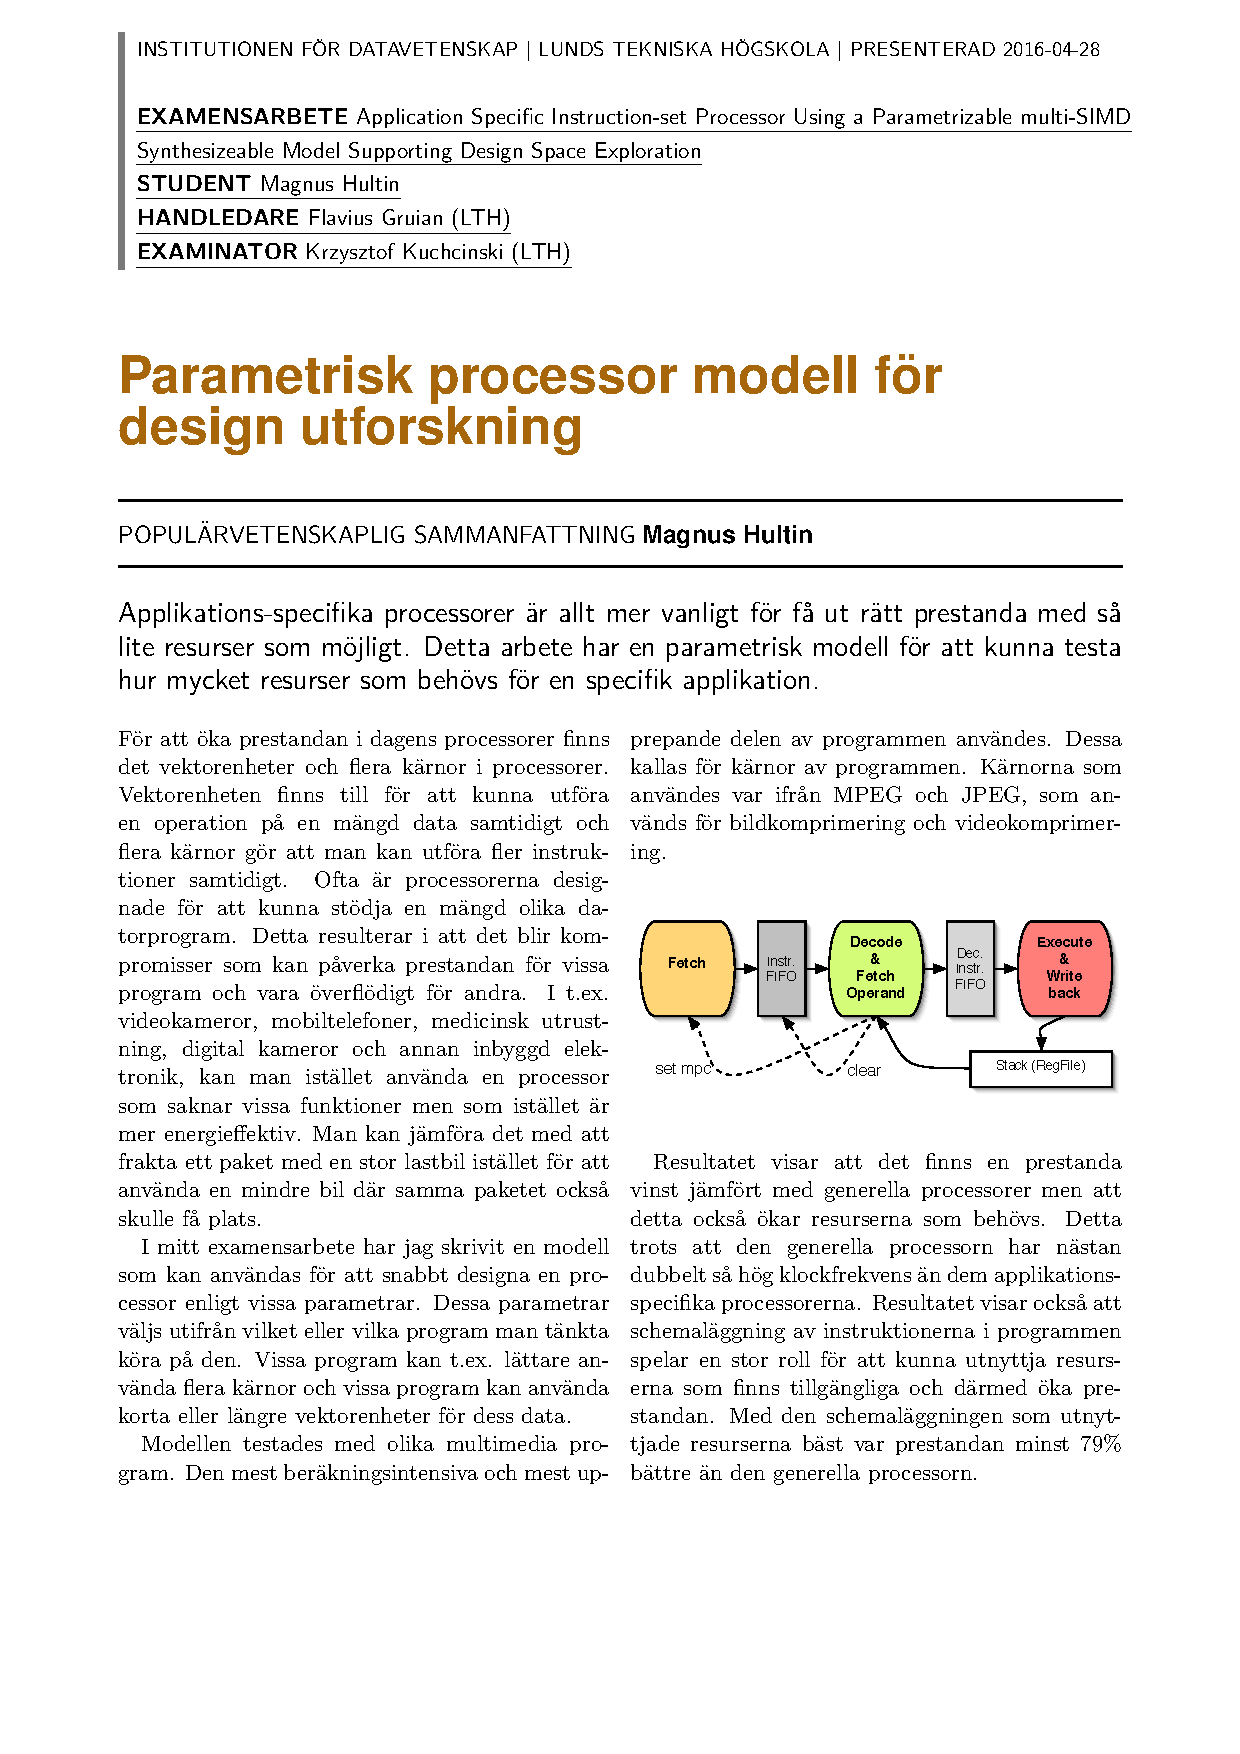
\includepdf[pages={1}]{popsci/popsci.pdf}
	%\end{appendices}

\end{document}
